\documentclass[a4paper,12pt]{report}
\usepackage[utf8]{inputenc} % style d'écriture
\usepackage[T1]{fontenc}      % package
\usepackage[francais]{babel}  % package pour langue française
\usepackage[a4paper]{geometry} % definition des marges
\usepackage[pdftex]{graphicx} % definition d'image
\usepackage{fancyhdr} % haut de page
\usepackage{float}
\usepackage{tcolorbox,listings}
\usepackage{caption}
\addtocounter{tocdepth}{3}
\setcounter{secnumdepth}{3}
\usepackage{color}
\usepackage{amssymb}

\lstset{
  aboveskip=5mm,
  belowskip=-2mm,
  basicstyle=\footnotesize,
  breakatwhitespace=false,
  breaklines=true,
  captionpos=b,
  commentstyle=\color{red},
  deletekeywords={...},
  escapeinside={\%*}{*)},
  extendedchars=true,
  framexleftmargin=16pt,
  framextopmargin=3pt,
  framexbottommargin=6pt,
  frame=tb,
  keepspaces=true,
  keywordstyle=\color{blue},
  language=VHDL,
  literate=
  {²}{{\textsuperscript{2}}}1
  {⁴}{{\textsuperscript{4}}}1
  {⁶}{{\textsuperscript{6}}}1
  {⁸}{{\textsuperscript{8}}}1
  {€}{{\euro{}}}1
  {é}{{\'e}}1
  {è}{{\`{e}}}1
  {ê}{{\^{e}}}1
  {ë}{{\"{e}}}1
  {É}{{\'{E}}}1
  {Ê}{{\^{E}}}1
  {û}{{\^{u}}}1
  {ù}{{\`{u}}}1
  {â}{{\^{a}}}1
  {à}{{\`{a}}}1
  {á}{{\'{a}}}1
  {ã}{{\~{a}}}1
  {Á}{{\'{A}}}1
  {Â}{{\^{A}}}1
  {Ã}{{\~{A}}}1
  {ç}{{\c{c}}}1
  {Ç}{{\c{C}}}1
  {õ}{{\~{o}}}1
  {ó}{{\'{o}}}1
  {ô}{{\^{o}}}1
  {Õ}{{\~{O}}}1
  {Ó}{{\'{O}}}1
  {Ô}{{\^{O}}}1
  {î}{{\^{i}}}1
  {Î}{{\^{I}}}1
  {í}{{\'{i}}}1
  {Í}{{\~{Í}}}1,
  morekeywords={*,...},
  numbers=left,
  numbersep=10pt,
  numberstyle=\tiny\color{black},
  rulecolor=\color{black},
  showspaces=false,
  showstringspaces=false,
  showtabs=false,
  stepnumber=1,
  stringstyle=\color{gray},
  tabsize=4,
  title=\lstname,
}

%\captionsetup[figure]{labelformat=empty}
\renewcommand{\thesection}{\Roman{section}}

\begin{document}
   \begin{titlepage}
    
    \newcommand{\HRule}{\rule{\linewidth}{0.5mm}} % Defines a new command for the horizontal lines, change thickness here
    
    \center % Center everything on the page
     
    %----------------------------------------------------------------------------------------
    %	HEADING SECTIONS
    %----------------------------------------------------------------------------------------
    
    \textsc{\LARGE Université de Bretagne Occidentale}\\[1.5cm] % Name of your university/college
		\textsc{\Large Master 2 Informatique}\\[0.5cm] % Major heading such as course name
		\textsc{\Large Département Informatique}\\[1.5cm] % Major heading such as course name
		{\large 2020/2021}\\[1.5cm] % Date, change the \today to a set date if you want to be precise
		
    \textsc{\large Vérification, Fiabilité et Sécurité}\\[1cm] % Minor heading such as course title
    
    %----------------------------------------------------------------------------------------
    %	TITLE SECTION
    %----------------------------------------------------------------------------------------
    
   \HRule \\[0.4cm]
    { \huge \bfseries Modélisation et prototypage avec AADLInspector/Ocarina d'un Système Embarqué}\\[0.2cm] % Title of your document
    \HRule \\[1cm]
     
    %----------------------------------------------------------------------------------------
    %	AUTHOR SECTION
    %----------------------------------------------------------------------------------------
    
    \begin{minipage}{0.48\textwidth}
			\begin{flushleft} \large
				\emph{Auteur:}\\
					William \textsc{PENSEC} % Your name
			\end{flushleft}
    \end{minipage}
		~
		\begin{minipage}{0.48\textwidth}
			\begin{flushright} \large
				\emph{Auteur:}\\
					Timothé \textsc{LANNUZEL} % Your name
			\end{flushright}
    \end{minipage}\\[1.5cm]
    
    %----------------------------------------------------------------------------------------
    %	DATE SECTION
    %----------------------------------------------------------------------------------------
    
    {\today}\\[1.5cm] % Date, change the \today to a set date if you want to be precise
    
    %----------------------------------------------------------------------------------------
    %	LOGO SECTION
    %----------------------------------------------------------------------------------------
    
		\begin{minipage}{0.48\textwidth}
			\begin{flushleft} \large
				
\includegraphics[scale=0.8]{ubo_sc.png} % Include a department/university logo - this will require the graphicx package
			\end{flushleft}
    \end{minipage}
		~
    \begin{minipage}{0.48\textwidth}
			\begin{flushright} \large
				
\includegraphics[scale=0.5]{ubo.png} % Include a department/university logo - this will require the graphicx package
			\end{flushright}
    \end{minipage}
    
    %----------------------------------------------------------------------------------------
    
    \vfill % Fill the rest of the page with whitespace
    
    \end{titlepage}
		
	\pagestyle{fancy}
		\lhead{William PENSEC \& Timothé LANNUZEL}
		\chead{}
		\rhead{Projet AADL}
		\lfoot{}
		\cfoot{\thepage}
		\rfoot{}
		
	\newpage\renewcommand{\contentsname}{Sommaire}
	\tableofcontents

	\newpage
	\section{Introduction}
		\paragraph*{}
		L'objectif de ce projet est de construire un modèle AADL à partir d'un système proposé dans une publication scientifique puis de tester le modèle sur AADLInspector et d'en faire une simulation avec l'outil Ocarina. La version utilisée pour AADLInspector est la version de démonstration sur Windows 10 et Ocarina est utilisé sur une machine virtuelle sur Linux (Ubuntu 16.04).
		
		Nous avons choisi l'article : "Platform-Based Embedded Software Design and System Integration for Autonomous Vehicles" de MM et Mme BENJAMIN HOROWITZ, JUDITH LIEBMAN, CEDRIC MA, T. JOHN KOO, ALBERTO SANGIOVANNI - VINCENTELLI et S. SHANKAR SASTRY. Ce document parle des drones autonomes et de leurs systèmes de navigation.
		
		\paragraph*{}
		Nous avons choisi de concevoir plusieurs versions du modèle afin de mieux montrer le système sous différentes possibilités d'interprétation et d'implémentation.
	
	\section{Description du système étudié}
		\paragraph*{}
		Afin d'étudier le système, nous avons mis en place la solution suivante (voir Figure \ref{archi}). Comme on peut le voir sur l'image\footnote{L'image présentée ici vient de l'article étudié et correspond à la Fig. 7 Refined Giotto program} et comme il est dit dans l'article, nous avons pris pour \texttt{THREADS} principaux \texttt{Fusion} et \texttt{Control} qui sont appellés respectivement \texttt{dataProc} et \texttt{controller} dans notre code. Ainsi, le thread \texttt{Fusion} va recevoir les valeurs du \texttt{GPS} et de l'\texttt{INS}, puis va les traiter et ensuite les envoyer au thread \texttt{Control} afin de transformer ces valeurs du \texttt{GPS} et de l'\texttt{INS} en une donnée compréhensible pour les servos servant à diriger l'appareil.
		

		\begin{figure}[H]
			\centering
				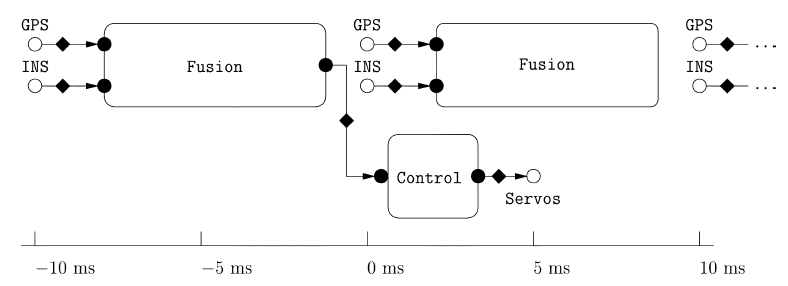
\includegraphics[scale=0.7]{archi.png}
				\caption{Système appliqué à notre solution}
			\label{archi}
		\end{figure}
			
		\paragraph*{}
		Nous avons, à partir de ce système, conçu 3 versions différentes qui seront détaillées dans la partie suivante. Chaque version correspond à une implémentation possible entre ce qui est mis dans l'article ou ce qui est apparu dans notre conception du système.
		
	\section{Description et explication du modèle AADL}
		\paragraph*{}
		Nous avons tenu à faire différentes versions du système car dans l'article ils mentionnaient plusieurs solutions et certains points n'étaient pas très clair.
		Par exemple, on peut citer les données manquantes telles que le temps de récupération des données venant du \texttt{GPS} et de l'\texttt{INS}. Sinon les données de la période du \texttt{Data Processor} et du \texttt{Time Based Controller} sont assez clair et il était expliqué dans l'article pourquoi ils prennaient les valeurs choisies.
		
		\paragraph*{}
		Une trace d'exécution sur AADLInspector est trouvable à la fin du fichier dans la partie \ref{traces} à la page \pageref{traces}.
		
		
		\subsection{Version 1}
			\paragraph*{}
			La première version est une version annexe avec 1 \texttt{CPU} et 5 threads. Ces threads sont :
			
			\begin{itemize}
				\item[$\blacktriangleright$] Un thread pour la gestion de l'envoi et de la réception des données (\texttt{dataProc})
				\item[$\blacktriangleright$] Un deuxième afin de formatter les données afin que les servos moteurs comprennent l'information et ce qu'ils doivent exécuter (\texttt{controller}).
				\item[$\blacktriangleright$] Un troisième qui gère le \texttt{GPS} (\texttt{device\_GPS}).
				\item[$\blacktriangleright$] Un quatrième qui gère l'\texttt{INS} (\texttt{device\_INS}).
				\item[$\blacktriangleright$] Un cinquième qui gère les \texttt{Servos} (\texttt{device\_SERVOS}).
			\end{itemize}
			
			\paragraph*{}
			Dans la figure \ref{v0}, les cadres en pointillés représentent les différents threads du système. Les threads des appareils physiques ne permettent que de communiquer entre l'appareil physique et le thread \texttt{dataProc} afin de recevoir des données.
			
			\begin{figure}[H]
				\centering
					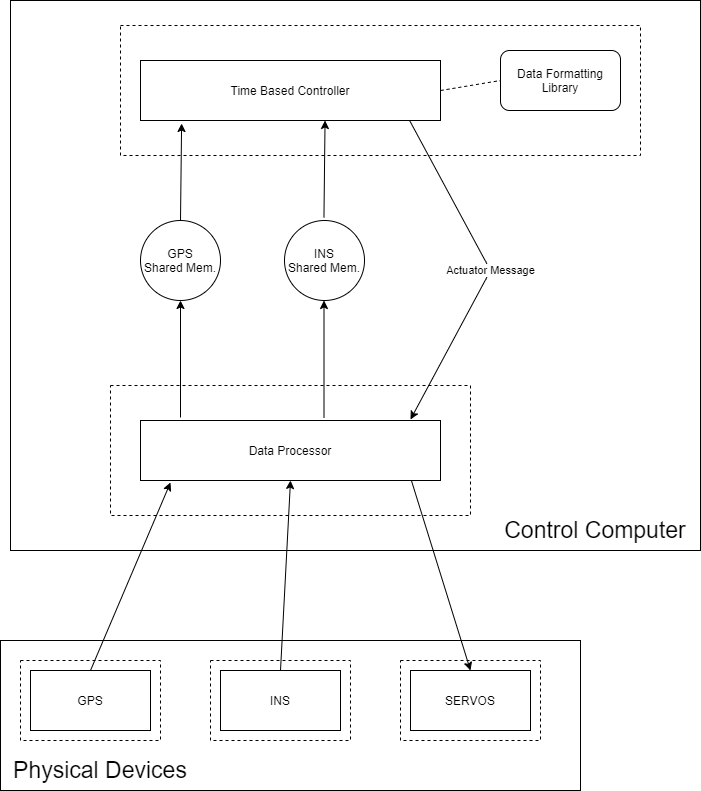
\includegraphics[scale=0.4]{v0.png}
					\caption{Système appliqué avec 1 CPU et 5 threads}
				\label{v0}
			\end{figure}
			
			
			\paragraph*{}
			Nous présentons à présent les différentes valeurs appliquées pour chacun des threads. Le fait de mettre un décalage seulement au \texttt{device\_Servos} permet qu'il démarre seulement après que le \texttt{dataProc} ait lu et envoyé la valeur du \texttt{controller} aux servos sinon il s'exécuterait pour rien et entrainerait donc une petite perte de performance. Pour calculer le décalage on prend le temps d'exécution du \texttt{dataProc} + celui du \texttt{controller}.
			
			\begin{table}[H]
			\centering
			\resizebox{\textwidth}{!}{%
				\begin{tabular}{|c|c|c|c|c|c|c|}
					\hline
																				 & Ordonnancement & Période  & Deadline & Temps d'exécution & Priorité & Décalage  	\\ \hline
					\textcolor{red}{dataProc} 		 & 	Périodique 		& 	20 ms	 &  20 ms		&  			0 à 10 ms		& 		9 	 & 						\\ \hline
					\textcolor{red}{controller} 	 & 	Périodique 	 	& 	20 ms	 &  20 ms		&  			0 à 5 ms		& 		8 	 & 						\\ \hline
					\textcolor{red}{device\_GPS} 	 & 	Périodique 	 	& 	20 ms	 &  20 ms		&  			0 à 1 ms		& 		8 	 & 						\\ \hline
					\textcolor{red}{device\_INS} 	 & 	Périodique 	 	& 	20 ms	 &  20 ms		&  			0 à 1 ms		& 		8 	 & 						\\ \hline
					\textcolor{red}{device\_Servos} & 	Périodique 	& 	20 ms	 &  20 ms		&  			0 à 1 ms		& 		8 	 & 		15 ms		\\ \hline
				\end{tabular}
			}
		\end{table}
			
		\subsection{Version 2}
			\paragraph*{}
			La deuxième version implémentée est une version avec 1 \texttt{CPU} qui prend en charge 2 threads : 
			
			\begin{itemize}
				\item[$\blacktriangleright$] Un thread pour la gestion de l'envoi et de la réception des données (\texttt{dataProc}).
				\item[$\blacktriangleright$] Un deuxième afin de formatter les données afin que les servos moteurs comprennent l'information et ce qu'ils doivent exécuter (\texttt{controller}).
			\end{itemize}
			
			L'image suivante\footnote{L'image présentée ici vient de l'article étudié et correspond à la Fig. 8 First implementation of UAV platform. The dashed line encloses the platform implementation.} montre le schéma d'architecture de cette version. Le \texttt{CPU} correspond au \texttt{Control Computer}.
			\begin{figure}[H]
				\centering
					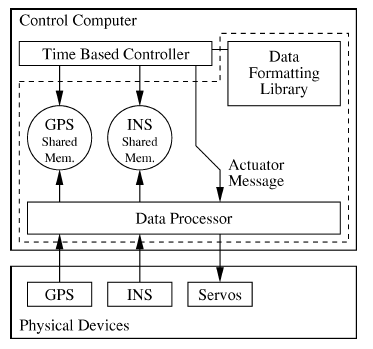
\includegraphics[scale=0.7]{cpu1.png}
					\caption{Système appliqué avec 1 CPU}
				\label{cpu1}
			\end{figure}
			
			
			\paragraph*{}
			Nous présentons à présent les différentes valeurs appliquées pour chacun des threads.
			
			\begin{table}[H]
			\centering
			\resizebox{\textwidth}{!}{%
				\begin{tabular}{|c|c|c|c|c|c|c|}
					\hline
																				 & Ordonnancement & Période  & Deadline & Temps d'exécution & Priorité 	\\ \hline
					\textcolor{red}{dataProc} 		 & 	Périodique 		& 	20 ms	 &  20 ms		&  			0 à 10 ms		& 		9			\\ \hline
					\textcolor{red}{controller} 	 & 	Périodique 	 	& 	20 ms	 &  20 ms		&  			0 à 5 ms		& 		8			\\ \hline
				\end{tabular}
			}
		\end{table}
		
		\paragraph*{}
		Actuellement, nous avons seulement implémenter cette version avec Ocarina et tout est fonctionnel. Nous avons implémenté cette version afin de montrer qu'il est possible d'envoyer des données et d'en recevoir avec une exécution correcte selon les périodes et temps d'exécution des tâches. Voici un exemple d'exécution du code une fois compilé avec Ocarina :
		
		\begin{figure}[H]
				\centering
					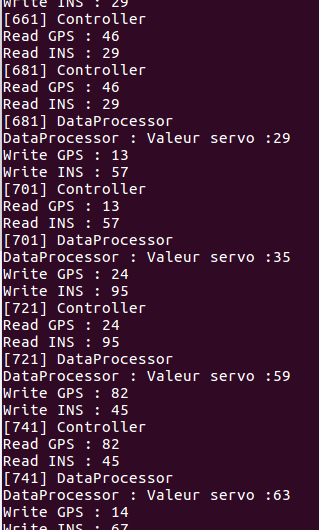
\includegraphics[scale=0.5]{ocarina.png}
					\caption{Exécution de la Version 2}
				\label{ocarina}
			\end{figure}
	
		\subsection{Version 3}
			\paragraph*{}
			La deuxième version implémentée est une version avec 2 \texttt{CPU} qui prennent chacun en charge 1 thread.
			
			\begin{itemize}
				\item[$\blacktriangleright$] Le premier \texttt{CPU} correspond au \texttt{Control Computer} qui permet de traiter les informations reçues du deuxième \texttt{CPU} avec les données du \texttt{GPS} et de l'\texttt{INS}; puis ensuite permet de renvoyer la valeur calculée au deuxième \texttt{CPU}.
			
				\item[$\blacktriangleright$] Le deuxième \texttt{CPU} correspond au \texttt{Data Computer} qui permet de récupérer les informations envoyées par le \texttt{GPS} et par l'\texttt{INS}. Puis envoyer ces valeurs au premier \texttt{CPU} qui va donc calculer puis ensuite une fois la valeur reçu du premier \texttt{CPU}, le \texttt{Data Computer} appelle la partie \texttt{Data Formatting Library} qui va rendre compréhensible la valeur pour les servos moteurs de l'appareil; et enfin, envoi cette valeur formatée aux servos.
			\end{itemize}
			
			L'image suivante\footnote{L'image présentée ici vient de l'article étudié et correspond à la Fig. 9 Second implementation of UAV platform. The dashed line encloses the platform implementation.} montre le schéma d'architecture de cette version. Le \texttt{CPU1} correspond au \texttt{Control Computer}, le \texttt{CPU2} correspond au \texttt{Data Computer} et les \texttt{Physical Devices} communiquent avec le \texttt{CPU2}.
			\begin{figure}[H]
				\centering
					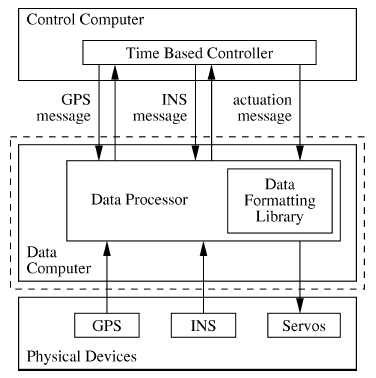
\includegraphics[scale=0.7]{cpu2.png}
					\caption{Système appliqué avec 2 CPU}
				\label{cpu2}
			\end{figure}
			
			
			\paragraph*{}
			Nous présentons à présent les différentes valeurs appliquées pour chacun des threads. Le fait de mettre un décalage seulement au controller permet qu'il démarre seulement après que le \texttt{dataProc} ait lu une valeur du GPS et de l'INS sinon il s'exécuterait pour rien et entrainerait donc une petite perte de performance. Pour calculer le décalage on prend le temps d'exécution du \texttt{dataProc} et c'est tout.
			
			\begin{table}[H]
			\centering
			\resizebox{\textwidth}{!}{%
				\begin{tabular}{|c|c|c|c|c|c|c|}
					\hline
																				 & Ordonnancement & Période  & Deadline & Temps d'exécution & Priorité & Décalage  	\\ \hline
					\textcolor{red}{dataProc} 		 & 	Périodique 		& 	20 ms	 &  20 ms		&  			0 à 10 ms		& 		9 	 & 						\\ \hline
					\textcolor{red}{controller} 	 & 	Périodique 	 	& 	20 ms	 &  20 ms		&  			0 à 5 ms		& 		8		 &	10 ms			\\ \hline
				\end{tabular}
			}
			\end{table}
			
	\section{Utilisations potentielles du modèle}
		\paragraph*{}
		Les vérifications que les modèles permettent de faire sont de simuler le système de navigation d'un véhicule autonome (type UAV) selon les données reçues des capteurs présents sur l'appareil comme par exemple le \texttt{GPS} et l'\texttt{INS}. Ces données, une fois traitées, permettent d'actionner ou non les servos moteurs de l'appareil afin de recalibrer la direction du drone. Les vérifications qui sont intéressantes et nécessaires de faire sont de vérifier que le modèle respecte bien les deadlines des tâches, en évitant que la somme des périodes des tâches soient supérieur à la capacité totale du CPU utilisé.
		
		
		\paragraph*{}
		Les paramètres ou données intéressants à déterminer pour le système étudié sont les périodes, deadline, temps d'exécution et ordre d'exécution des tâches (\texttt{dataProc} et \texttt{controller}) afin de garantir un bon fonctionnement du système et éviter les malfonctionnements.
		
		
		
	\section{Annexes : traces sur AADLInspector}
		\label{traces}
	
		\begin{figure}[H]
			\centering
				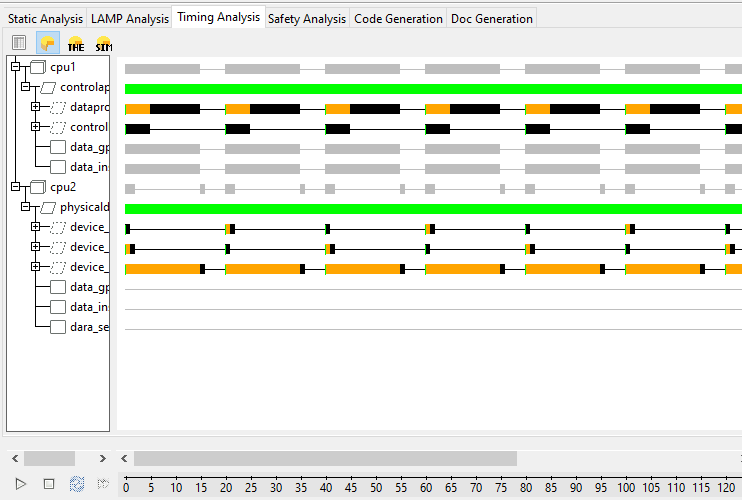
\includegraphics[scale=0.5]{execV1.png}
				\caption{Trace d'exécution de la Version 1 du système}
			\label{execV1}
		\end{figure}
		
		\begin{figure}[H]
			\centering
				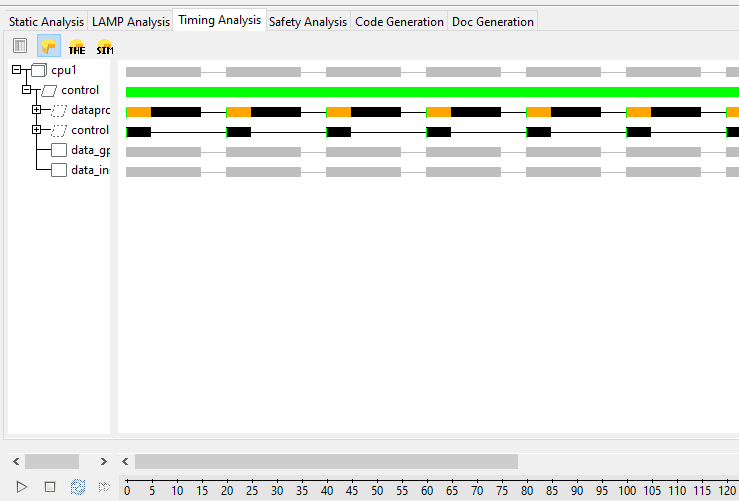
\includegraphics[scale=0.5]{execV2.png}
				\caption{Trace d'exécution de la Version 2 du système}
			\label{execV2}
		\end{figure}
		
		\begin{figure}[H]
			\centering
				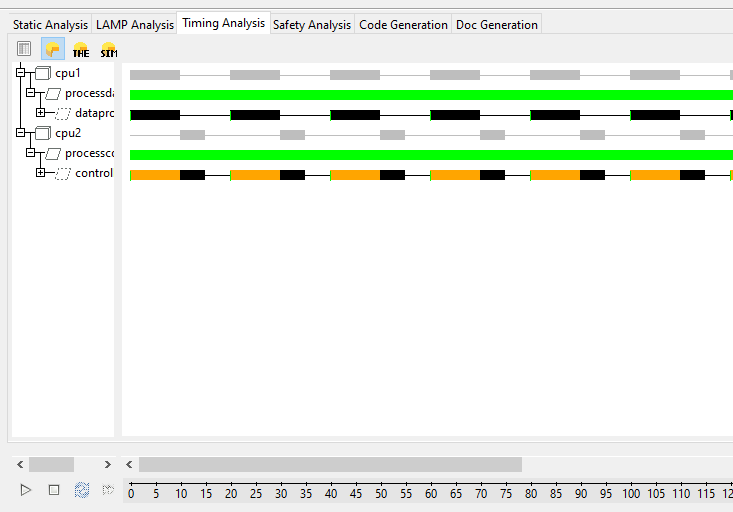
\includegraphics[scale=0.5]{execV3.png}
				\caption{Trace d'exécution de la Version 3 du système}
			\label{execV3}
		\end{figure}
	
	
	\clearpage
\end{document}